% SIAM Article Template
\documentclass[review,onefignum,onetabnum]{siamonline250106}

% Information that is shared between the article and the supplement
% (title and author information, macros, packages, etc.) goes into
% ex_shared.tex. If there is no supplement, this file can be included
% directly.

% SIAM Shared Information Template
% This is information that is shared between the main document and any
% supplement. If no supplement is required, then this information can
% be included directly in the main document.


% Packages and macros go here
\usepackage{lipsum}
\usepackage{amsfonts}
\usepackage{graphicx}
\usepackage{epstopdf}
\usepackage{soul}
\usepackage{caption}
\usepackage{subcaption}
\usepackage{algorithm}
\usepackage{algpseudocode}
\usepackage{enumitem}
\usepackage{comment}
\ifpdf
  \DeclareGraphicsExtensions{.eps,.pdf,.png,.jpg}
\else
  \DeclareGraphicsExtensions{.eps}
\fi

% \usepackage[dvipsnames,x11names]{xcolor}

\usepackage{booktabs}
\usepackage{multirow}
\usepackage{annotate-equations}

% Prevent itemized lists from running into the left margin inside theorems and proofs
\usepackage{enumitem}
\setlist[enumerate]{leftmargin=.5in}
\setlist[itemize]{leftmargin=.5in}

% Add a serial/Oxford comma by default.
\newcommand{\creflastconjunction}{, and~}

% Used for creating new theorem and remark environments
\newsiamremark{remark}{Remark}
\newsiamremark{hypothesis}{Hypothesis}
\crefname{hypothesis}{Hypothesis}{Hypotheses}
\newsiamthm{claim}{Claim}

% Sets running headers as well as PDF title and authors
% \headers{Utilizing Covariance Uncertainty in Multi-fidelity Estimation with Approximate Control Variates}{T. Coons, A. Jivani, and X. Huan}

\headers{SVGD Notes}{A. Jivani, T. Coons and X. Huan}

% Title. If the supplement option is on, then "Supplementary Material"
% is automatically inserted before the title.
% \title{Utilizing Covariance Uncertainty in Multi-fidelity Estimation with Approximate Control Variates\thanks{Submitted to the editors DATE.
% \funding{Enter funding sources!}}}
\title{Research Notes (Scalable SVGD)}

% Authors: full names plus addresses.
\author{AJ}

\usepackage{amsopn}
\DeclareMathOperator{\diag}{diag}


%%%% HELPER CODE FOR DEALING WITH EXTERNAL REFERENCES ON OVERLEAF
% (from an answer by cyberSingularity at http://tex.stackexchange.com/a/69832/226)
%%%
\makeatletter
\newcommand*{\addFileDependency}[1]{% argument=file name and extension
  \typeout{(#1)}% latexmk will find this if $recorder=0 (however, in that case, it will ignore #1 if it is a .aux or .pdf file etc and it exists! if it doesn't exist, it will appear in the list of dependents regardless)
  \@addtofilelist{#1}% if you want it to appear in \listfiles, not really necessary and latexmk doesn't use this
  \IfFileExists{#1}{}{\typeout{No file #1.}}% latexmk will find this message if #1 doesn't exist (yet)
}
\makeatother

\newcommand*{\myexternaldocument}[1]{%
    \externaldocument{#1}%
    \addFileDependency{#1.tex}%
    \addFileDependency{#1.aux}%
}
%%% END HELPER CODE

%%% Local Variables: 
%%% mode:latex
%%% TeX-master: "ex_article"
%%% End: 



% % SIAM Shared Information Template
% % This is information that is shared between the main document and any
% % supplement. If no supplement is required, then this information can
% % be included directly in the main document.


% % Packages and macros go here
% \usepackage{lipsum}
% \usepackage{amsfonts}
% \usepackage{graphicx}
% \usepackage{epstopdf}
% \usepackage{algorithmic}
% \ifpdf
%   \DeclareGraphicsExtensions{.eps,.pdf,.png,.jpg}
% \else
%   \DeclareGraphicsExtensions{.eps}
% \fi

% % Prevent itemized lists from running into the left margin inside theorems and proofs
% \usepackage{enumitem}
% \setlist[enumerate]{leftmargin=.5in}
% \setlist[itemize]{leftmargin=.5in}

% % Add a serial/Oxford comma by default.
% \newcommand{\creflastconjunction}{, and~}

% % Used for creating new theorem and remark environments
% \newsiamremark{remark}{Remark}
% \newsiamremark{hypothesis}{Hypothesis}
% \crefname{hypothesis}{Hypothesis}{Hypotheses}
% \newsiamthm{claim}{Claim}

% % Sets running headers as well as PDF title and authors
% \headers{Multi-fidelity SVGD}{A. Jivani, T. Coons, X. Huan}

% % Title. If the supplement option is on, then "Supplementary Material"
% % is automatically inserted before the title.
% % \title{An Example Article\thanks{Submitted to the editors DATE.
% % \funding{This work was funded by the Fog Research Institute under contract no.~FRI-454.}}}

% \title{Scalable Stein Variational Gradient Descent via Multifidelity Particle Transport with Application to Bayesian Inference\thanks{Submitted to the editors DATE.
% \funding{This work is supported in part by the National Science Foundation Graduate Research Fellowship under Grant No. DGE 1841052, the Department of Navy award N00014-23-1-2735 issued by the Office of Naval Research, and through computational resources and services provided by Advanced Research Computing at the University of Michigan, Ann Arbor.}}}

% % Authors: full names plus addresses.
% \author{Aniket Jivani \thanks{Department of Mechanical Engineering, University of Michigan, Ann Arbor, MI, 48109 
%   (Correspondence: \email{ajivani@umich.edu}).}
% \and Thomas E. Coons \footnotemark[2]
% \and Xun Huan \footnotemark[2]}

% \usepackage{amsopn}
% \DeclareMathOperator{\diag}{diag}


% %%%% HELPER CODE FOR DEALING WITH EXTERNAL REFERENCES ON OVERLEAF
% % (from an answer by cyberSingularity at http://tex.stackexchange.com/a/69832/226)
% %%%
% \makeatletter
% \newcommand*{\addFileDependency}[1]{% argument=file name and extension
%   \typeout{(#1)}% latexmk will find this if $recorder=0 (however, in that case, it will ignore #1 if it is a .aux or .pdf file etc and it exists! if it doesn't exist, it will appear in the list of dependents regardless)
%   \@addtofilelist{#1}% if you want it to appear in \listfiles, not really necessary and latexmk doesn't use this
%   \IfFileExists{#1}{}{\typeout{No file #1.}}% latexmk will find this message if #1 doesn't exist (yet)
% }
% \makeatother

% \newcommand*{\myexternaldocument}[1]{%
%     \externaldocument{#1}%
%     \addFileDependency{#1.tex}%
%     \addFileDependency{#1.aux}%
% }
% %%% END HELPER CODE

% %%% Local Variables: 
% %%% mode:latex
% %%% TeX-master: "ex_article"
% %%% End: 


% Optional PDF information
\ifpdf
\hypersetup{
  pdftitle={SVGD Notes},
  % pdfauthor={A. Jivani, T. Coons, and X. Huan}
}
\fi

% The next statement enables references to information in the
% supplement. See the xr-hyperref package for details.

%% Use \myexternaldocument on Overleaf
\myexternaldocument{ex_supplement}

% FundRef data to be entered by SIAM
%<funding-group>
%<award-group>
%<funding-source>
%<named-content content-type="funder-name"> 
%</named-content> 
%<named-content content-type="funder-identifier"> 
%</named-content>
%</funding-source>
%<award-id> </award-id>
%</award-group>
%</funding-group>

% \documentclass[12pt]{article}
% \usepackage{graphicx} % Required for inserting images
% \usepackage[utf8]{inputenc}

%%% tikz & libraries
\usepackage{tikz}
\usepackage{multirow}
\usetikzlibrary{backgrounds}
\usetikzlibrary{arrows,shapes}
\usetikzlibrary{tikzmark} % for \tikzmarknode
% \usetikzlibrary{calc} % for computing the midpoint between two nodes, e.g. at ($(p1.north)!0.5!(p2.north)$) 

% Commands for Highlighting text -- non tikz method
\newcommand{\highlight}[2]{\colorbox{#1!17}{$#2$}}
\newcommand{\highlightdark}[2]{\colorbox{#1!47}{$#2$}}
%%% NOTE: \colorbox sets the second argument in text mode, so for use within equations we wrap it in $ $ again
% if you use \highlight or \highlightdark in subscripts, you need to pass \scriptstyle to get the font size right
% e.g. $ \mathbb{E}_{\highlight{BurntOrange}{\scriptstyle y}} $
\usepackage{annotate-equations}

% Colors that are more readable for comments
\definecolor{darkred}{rgb}{.7,0,0}
\newcommand\Red[1]{\textcolor{darkred}{#1}}
\definecolor{darkgreen}{rgb}{.15,.55,0}
\newcommand\Green[1]{\textcolor{darkgreen}{#1}}
\definecolor{darkblue}{rgb}{0,0,0.7}
\newcommand\Blue[1]{\textcolor{darkblue}{#1}}



\newcommand{\xh}[1]{\textcolor{orange}{\textbf{(XH:)} #1}}
\newcommand{\xhtd}[1]{\todo[linecolor=orange,backgroundcolor=orange!25]{#1}}
\newcommand{\tc}[1]{\textcolor{blue}{\textbf{(TC:)} #1}}
\newcommand{\aj}[1]{\textcolor{violet}{\textbf{(AJ:)} #1}}

% Variables.
\newcommand{\design}{\xi}
\newcommand{\Design}{\Xi}
\newcommand{\pdf}{p}
\newcommand{\policy}{\pi}
\newcommand{\info}{I}
\newcommand{\param}{\theta}
\newcommand{\Param}{\Theta}
\newcommand{\paramset}{\bm{\Theta}}
\newcommand{\noise}{\epsilon}
\newcommand{\Noise}{\mathcal{E}}
\newcommand{\ExpLoss}{\overline{\mathcal{L}}}


% Operators. 
\newcommand{\Var}{\mathbb{V}\text{ar}}
\newcommand{\Cov}{\mathbb{C}\text{ov}}
\newcommand{\DKL}{D_{\text{KL}}}
\newcommand{\tr}{\text{tr}}
\newcommand{\argmax}{\operatornamewithlimits{argmax}}
\newcommand{\argmin}{\operatornamewithlimits{argmin}}
\newcommand{\normdist}{\mathcal{N}}


% mathcal
\newcommand{\CA}{\mathcal{A}}
\newcommand{\CD}{\mathcal{D}}
\newcommand{\CF}{\mathcal{F}}
\newcommand{\CH}{\mathcal{H}}
\newcommand{\CM}{\mathcal{M}}
\newcommand{\CN}{\mathcal{N}}
\newcommand{\CS}{\mathcal{S}}
\newcommand{\CX}{\mathcal{X}}
\newcommand{\CL}{\mathcal{L}}


% mathbb
\newcommand{\EE}{\mathbb{E}}
% \newcommand{\PP}{\mathbb{P}}
\newcommand{\RR}{\mathbb{R}}
\newcommand\prob{\mathbb{P}}
\newcommand{\PP}{\mathbb{P}}

% mathbf
\newcommand{\bd}{\mathbf{d}}
\newcommand{\bg}{\mathbf{g}}
\newcommand{\bDelta}{\mathbf{\Delta}}

% hat
\newcommand{\hx}{\hat{x}}
\newcommand{\hg}{\hat{g}}
\newcommand{\hh}{\hat{h}}

% bar
\newcommand{\barh}{\bar{h}}


\DeclareMathOperator\supp{supp}
\newcommand{\etal}{\textit{et al.}}

% \newcommand{\Var}{\textrm{Var}}
% \newcommand{\Cov}{\textrm{Cov}}


% algorithms
\renewcommand{\algorithmicrequire}{\textbf{Input:}}
\renewcommand{\algorithmicensure}{\textbf{Output:}}



% Used Section 3.2 Onwards (can change names based on terms)
% \colorlet{colorp}{NavyBlue}
% \colorlet{colorT}{WildStrawberry}
% \colorlet{colork}{OliveGreen}
% \colorlet{colorM}{RoyalPurple}
% \colorlet{colorNb}{Plum!80}
% \colorlet{colorIs}{black}
% \colorlet{customrgbgreen}{darkgreen}
% % \colorlet{colorY}{goldenrod}
% \colorlet{colorY}{Dandelion}

\usepackage{hyperref}

\hypersetup{
  colorlinks=true,
  citecolor=blue,
  linkcolor=red,
  urlcolor=magenta,
  }

\usepackage{float}
\usepackage{url}
\usepackage{tabularx}
\usepackage{amsmath}
\usepackage{amsfonts}
\usepackage{amssymb}
\usepackage{mathtools}
\usepackage{xurl}
\usepackage{lineno}
\usepackage{epsfig}

\usepackage{ulem}
\newcommand{\stkout}[1]{\ifmmode\text{\sout{\ensuremath{#1}}}\else\sout{#1}\fi}
\usepackage{multirow}
\usepackage{longtable}
\setlength\LTleft{0pt}
\usepackage{tabularx}
\usepackage{epsfig}
\usepackage[numbers]{natbib}


% \newcommand{\xh}[1]{\textcolor{orange}{\textbf{(xh:)} #1}}
% \newcommand{\tc}[1]{\textcolor{red}{\textbf{(tc:)} #1}}
% \newcommand{\aj}[1]{\textcolor{magenta}{\textbf{(aj:)} #1}}

\begin{document}
\maketitle


% \begin{keywords}
%   example, \LaTeX
% \end{keywords}

% % REQUIRED
% \begin{AMS}
%     62K99, 68T07
% \end{AMS}


% \section{Introduction}

% \section{Background and Related Work}



\section{Stein Variational Gradient Descent}\label{ss: svgd}

Bayesian inference is a rigorous and general framework for reasoning under uncertainty: we construct a full probability model for all observable and unobservable quantities in a problem, followed by conditioning on the observed data to characterize the posterior distribution for the unobserved quantities. We provide a brief description below:

Let $\theta$ denote an unobservable quantity or parameter, and $D$ denote data or \textit{observations} collected through experiments or simulations. In order to estimate $\theta$, we define and decompose a joint probability distribution on $\theta$ and $D$ as follows:
\begin{align}
    p(\theta, D) = \underbrace{p(\theta)}_{\text{prior}} \underbrace{p(D\mid\theta)}_{\text{likelihood}}
\end{align}

The object of interest in Bayesian inference is the ``posterior density'' $p(\theta \mid D)$, which is the updated uncertainty for the unknown parameters conditioned on the newly acquired observations. It is obtained through the re-arrangement of the various conditional probabilities and summarized via Bayes' theorem:

\begin{align}
    p(\theta \mid D) = \frac{p(D\mid\theta) \, p(\theta)}{p(D)},
    \label{eqn: bayes_rule_v1}
\end{align}

where $p(D)$ is the evidence or marginal likelihood, and often intractable quantity that acts as a normalizing constant on the often tractable likelihood and prior.

Markov Chain Monte Carlo (MCMC) methods \citep{brooks_handbook_2011} are considered a workhorse of modern statistical inference. 
The high-level idea is to generate a sequence of random samples through construction of a Markov chain whose equilibrium distribution is the target posterior distribution. 
In addition to sampling from arbitrary distribution families, it also has the key benefit of asymptotic convergence guarantees. 
However, these methods are computationally intensive when dealing with high-dimensional parameter spaces, despite some impressive algorithmic advancements that make use of gradient information to guide new proposals.

Variational Inference (VI)\citep{jordan_introduction_1999,blei_variational_2017} reformulates traditional Bayesian inference as an optimization problem, where the posterior is approximated by a parametric family of distributions that is closest to the true posterior through a suitable measure. This is usually the reverse KL divergence or other measures from the family of $f$-divergence between probabiliy distributions. 
While VI is much more scalable to higher-dimensional spaces compared to MCMC, this scalability often trades off its approximation capacity, which is constrained by the choice of the variational family. 
For instance, mean-field variational Bayes assumes factorization of the variational distribution into independent variational approximations over each latent variable. 
However, dependencies between the hidden variables mean that this family typically does not contain the true posterior distribution. 
In general, VI can result in biased approximations to the posterior.

Stein Variational Gradient Descent (SVGD), introduced in \cite{Liu2016}, proposes a powerful non-parametric VI method. First, a transport map $T$ is defined between a tractable reference distribution $q_0(x)$ and the target density. 
Rather than restricting the set of transforms $T$ to a certain parametric form, it is instead constructed incrementally to propagate an initial set of particles drawn from $q_0$, with each successive transform directed towards steepest rate of change of KL divergence. 

SVGD falls into a class of methods making use of gradient flows of various divergence measures to sample from a target density in generative modeling. It is based on gradient flow of KL divergence over the $\CH$-Wasserstein distance, where $\CH$ is an RKHS equipped with kernel $k(x, x')$. 
This is exploited to result in a deterministic, interpretable and simple inference procedure resembling gradient descent. 
It can be used to characterize complex posterior distributions and is easily parallelizable. Subsequent developments \citep{mroueh_sobolev_2019,korba_kernel_2021} have led to competetive transport methods based on gradient flow of other discrepancy measures such as the MMD, and the kernelized Stein discrepancy (KSD).

% Stein's method has been applied to a measure transport framework under arbitrary transport map parametrization \citep{fisher_measure_2021}, using the Kernelized Stein Discrepancy (KSD) \citep{liu_kernelized_2016} as the objective instead of the traditional KL divergence. The curse of dimensionality in the kernel representation has also been tackled through the lens of projected transport \citep{chen_projected_2020}, that only propagates low-dimensional projection coefficients to the posterior.

Vanilla SVGD takes as input the target density function $p(x)$ and a set of initial particles $\{x_i^0\}_{i=1}^{n} \sim q_0(x)$ and returns a set of particles $\{x_i^L\}_{i=1}^{n}$ after L iterations that approximates the target distribution.

For iteration $l$, we update the particle positions via:

\begin{align}
    x_i^{l + 1} &\leftarrow x_i^l + \epsilon_l\hat{\phi}^{\ast}(x_i^l)\nonumber\\
    \text{ where }\hat{\phi}^{\ast}(x) &= \frac{1}{n}\left[\sum_{j=1}^n k(x_j^l, x) \nabla_{x_j^l}\log p(x_j^l) + \nabla_{x_j^l}k(x_j^l, x)\right]
    \label{eq: vanilla_svgd}
\end{align}

This is the decomposable Langevin-Stein operator. For a continuously differentiable and smooth target density, the decomposition involves the sum of $L$ operators, each of which acts on a single datapoint. The first term drives the particles towards regions towards the high probability regions of the posterior distribution, while the second term acts as a repulsive force that prevents mode collapse.

Notably, the convergence to the target density / fixed point of the system is decoupled from the update procedure itself, which only requires the perturbation direction to be aligned with the action of the Langevin-Stein operator. 
The vanilla SVGD procedure is naturally sensitive to choices of initial conditions, optimization methods, and hyperparameters such as the choice of kernel and the step size / learning rate sequence, used to find the fixed point. 
Common implementations of SVGD, including that of \cite{Liu2016} use Adagrad to set a per-parameter learning rate. The follow-up work of \cite{wang_stein_2019} generalizes the SVGD to make use of flexible matrix-valued kernels in gradient descent preconditioned with Hessian or Fisher information. These are complemented by learning-rate free methods, for example, the betting-strategy based \texttt{CoinSVGD} from \cite{sharrock_coin_2023}.

% Some remarks about the connection of SVGD to MCMC methods are in order. 
SVGD differs from conventional gradient-based MCMC methods in its evolution of a co-ordinated particle ensemble instead of simulation of Markov chains with individual particles. An example of the latter is Euler-discretized unadjusted Langevin algorithm (ULA). ULA is not equipped with a repulsive mechanism to ensure coverage, rather, Gaussian noise is injected at each step to prevent collapse to the MAP solution. 

% Stein's identity has also aided the construction of a useful discrepancy measure, the so-called Kernelized Stein Discrepancy (KSD), which finds use not only in goodness-of-fit statistical tests \citep{chwialkowski_kernel_2016}, but has also been extended to a measure transport framework under arbitrary transport map parametrization and an unbiased estimator of the score\citep{fisher_measure_2021}.

Independent of the update procedure and the hyperparameters, the major bottlenecks associated with transporting the particles are:

\begin{enumerate}
    \item Computing the gradient $\nabla_x \log p(x)$. For Bayesian Inference, this amounts to evaluating the score function associated with the posterior distribution and thereby the cost of repeated likelihood evaluations via a high-fidelity model.

    \item The $O(n^2)$ cost associated with computing elements $k(x_i, x_j)$ of the dense kernel matrix. \label{it: kernel_cost}
\end{enumerate}

The recommendation of \cite{Liu2016} is to approximate the score with subsampled mini-batches of the data, with a view to reduce the number of score evaluations at a single point $x$. A formal justification of this procedure appears in \cite{gorham_stochastic_2020}, where the stochastic Stein discrepancy is formulated and shown to converge to continuous SVGD in 1-Wasserstein distance. While these can bring about significant computational savings, they form a class of single-fidelity SVGD variants and do not consider reduction in cost of an individual forward model evaluation that underlies the likelihood definition.


The kernel weighting factor as well as the particle repulsion term also have scope for cost savings through identification of covariance structures as the map is iteratively constructed. 
One simple example is propagation of an initial set of particles towards a bimodal target density, visualized in Figure~\ref{fig:cov_structure}. 
Since particles assume memberships of separate clusters, this introduces some structure and potentially sparsity in the covariance matrix, which may be exploited to bring down the total kernel evaluation cost. 
Estimation of sparse covariance structures \citep{fop_model-based_2018} is of great interest in the statistical literature and in studies of  graphical models. 
For instance, a message-passing version of SVGD \citep{wang_stein_2018} is tailored to continuous graphical models through localized kernel approximations. 

\begin{figure}[htbp]
    \centering
    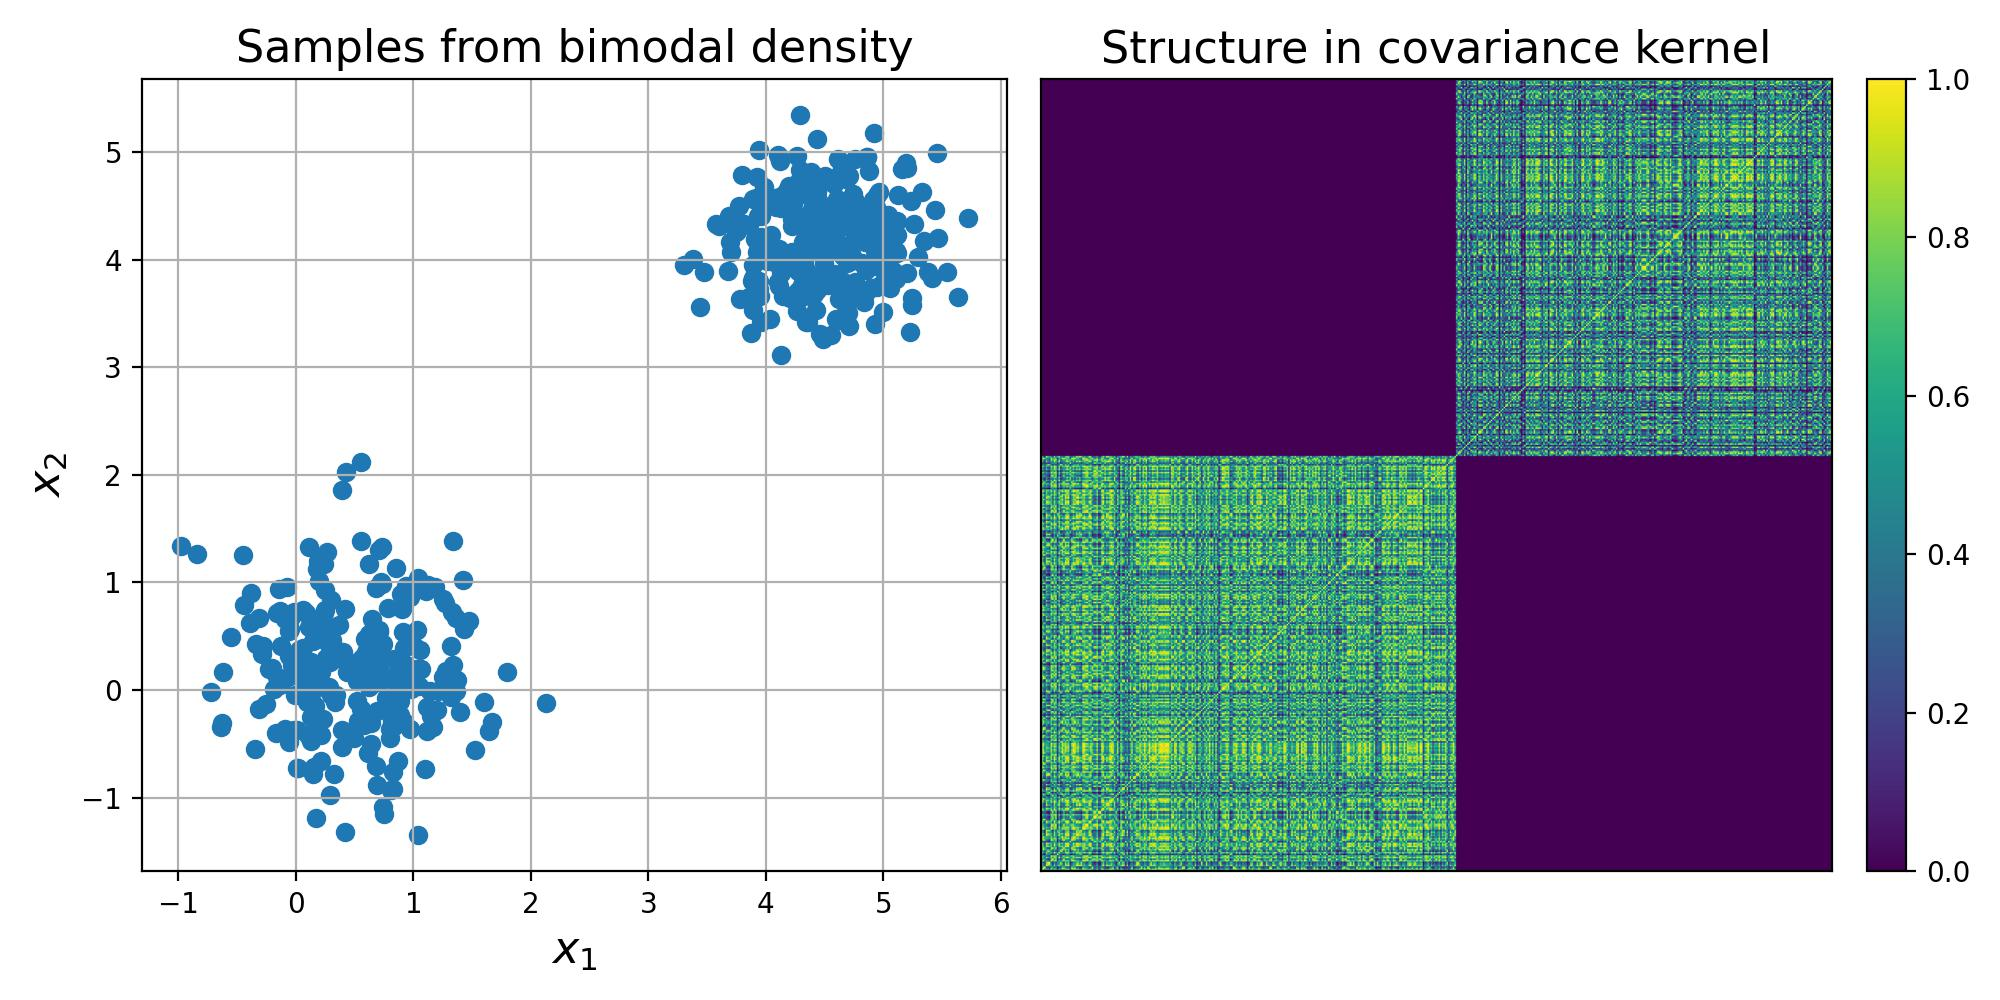
\includegraphics[width=0.75\linewidth]{figures/structure_cov_kernel.jpg}
    \caption{Covariance kernel with block diagonal structure corresponding to particles sampled from a bimodal target density}
    \label{fig:cov_structure}
\end{figure}

Our initial focus is on efficient evaluation of the score function through multi-fidelity setups that reduce the number of high-fidelity model-based likelihood evaluations, before considering a potential combination of the kernel and score approximation for future work.

% \subsection{Gradient-based MCMC Methods}

% SVGD differs from conventional gradient-based MCMC methods in its evolution of a co-ordinated particle ensemble instead of simulation of Markov chains with individual particles. In particular, the Euler-discretized Langevin dynamics simulates a Markov chain with the rule:

% \begin{equation}
%     x_{i+1} \leftarrow x_i + \frac{\epsilon}{2}\nabla \log p(x_i) + \epsilon \eta_i
% \end{equation}

% where $\eta_i \sim \CN(0, \epsilon)$ injects Gaussian noise at each step to prevent collapse to the MAP solution. 
% For Bayesian inference, Stochastic Gradient Langevin Dynamics (SGLD) \citep{welling_bayesian_2011,brosse_promises_2018} permits use of large-scale datasets through unbiased gradient estimators based on small mini-batches of the data, potentially augmented with control-variates for variance reduction. 
% While these approaches to Langevin dynamics are extremely relevant to discussions of variance reduction techniques for MCMC methods, the key ideas do not translate directly to the SVGD setting: instead of distributing workload amongst an ensemble of particles, these reduce the costs of likelihood evaluation conditioned on a particular realization of parameters $x$.


\section{Approximate Control Variates for Multi-fidelity Estimation}\label{ss: acv}

% \textcolor{red}{Stealing the text from acv with uq with some cuts}

Consider a mapping $Q=f_0(Z)$ that relates the random vector $Z \in \mathbb{R}^{n_{z}}$ and the random variable $Q \in \mathbb{R}$. The expected value of $Q$ is often approximated by a standard $N$-sample Monte Carlo (MC) estimator:
\begin{align}\label{eqn:mc}
    \mathbb{E}\left[Q_0\right] 
    \approx \hat{Q}_0 := \frac{1}{N} \sum^{N}_{j=1}f_0(z^{(j)}),
\end{align}

where $z^{(j)} \sim p(Z)$ are independent and identically distributed (i.i.d.) samples drawn from the probability distribution of $Z$. The MC estimator $\hat{Q}$ is unbiased, making its estimator error contributed entirely by its variance $N^{-1}\Var[Q]$. When using computationally intensive models, the number of samples $N$ that can be afforded may not be sufficiently high to limit this variance.

To reduce the estimator variance, multi-fidelity methods leverage an ensemble of low-fidelity models whose outputs are correlated with the high-fidelity model of interest but with diminished costs. 

Control variates (CVs) are a widely used classical method for variance reduction in Monte-Carlo methods. 
The general approach is to identify another function $f_1$, such that the traditional expected value estimator described in Equation~\ref{eqn:mc} can be replaced by one constructed with $f_0 - f_1$, with smaller variance. The function $f_1$ is then referred to as a control variate. 
Typically, selection of $f_1$ (generalized to selection of $\{f_i\}, i=1, \cdots, M$) and identifying a rich set of candidate CVs is a non-trivial procedure barring the exceptions where CVs can be identified from domain knowledge. 
Linear transformations of the score function have been one of the popular choices given the high canonical correlations with the target that result in better variance reduction, and their straightforward incorporation into modern MCMC methods with gradient information and marginalization of hyperparameters \citep{papamarkou_zero_2014,oates_control_2017}. \cite{si_scalable_2021} extends CV identification to the high-dimensional settings by proposing a variational formulation based on Stein operators.
% \footnote{\textcolor{red}{Technically these are control functionals rather than control variates? \citep{oates_control_2017}}}.


In the context of multifidelity methods however, we typically already have access to a hierarchy of models, where each available low-fidelity model can be leveraged as a control variate, but their respective expectations must be computed from samples too. The approximate control variate (ACV) technique \cite{Gorodetsky2020, bomarito_optimization_2022} provides a rigorous formulation for deriving reduced-variance estimators in this setting.
This method introduces $M$ auxiliary random variables $Q_{m}$ for $m=1,\ldots,M$ that are outputs of the corresponding (e.g., low-fidelity) models $Q_{m} =f_{m}(Z)$, then combines the corresponding MC estimates of each low-fidelity model, $\hat{Q}_{m}$, into a single estimator. The ACV estimator, which we denote $\tilde{Q}$, can be written as:
\begin{align}
        \Tilde{Q}(z,\alpha,\CA) &:= 
        \hat{Q}_{0}(z_{0})+\sum^{M}_{m=1}\alpha_{m}\left( \hat{Q}_{m}(z^{\ast}_{m})-\hat{\mu}_{m}(z_{m}) \right) \nonumber\\ 
        &= \hat{Q}_{0}(z_{0})+\sum^{M}_{m=1}\alpha_{m}\left( \hat{Q}_{m}(z^{\ast}_{m})-\hat{Q}_{m}(z_{m}) \right),     \label{eqn:ACV-Formula}
\end{align}
where $\hat{\mu}_{m}$ is an MC estimate for the $m$th model mean, $\alpha = \left[ \alpha_{1}, \ldots, \alpha_M \right]$ is a vector of control variate weights, and the input samples $z$ are partitioned into subsets $z_{0}$, $z_{m}$, and  $z^{\ast}_{m}$ according to a sample partitioning strategy $\CA$. The control variate weights $\alpha$ and the sample partitioning strategy $\CA$ are hyperparameters of the estimator.
%that are chosen to optimally reduce the estimator variance. 

Since the ACV estimator is unbiased with respect to the high-fidelity model, its error is equal to the estimator variance. To express this variance mathematically, we introduce a vectorized notation for the ACV estimator:
\begin{align}\label{eqn:vectorized-acv}
    \Tilde{Q}(z;\alpha,\CA) = \hat{Q}_{0} + \alpha^{\top}\Delta,
\end{align}
where $\Delta:=\left[ \Delta_{1}(z_{1}^{\ast},z_{1}), \ldots,  \Delta_{M}(z_{M}^{\ast},z_{M})\right]$, $\Delta_{m}(z_{m}^{\ast},z_{m}):=\hat{Q}_{m}(z^{\ast}_{m})-\hat{Q}_{m}(z_{m})$, and the explicit dependence on the inputs $z_{m}$ and $z_{m}^{\ast}$ are omitted for simplicity of notation. The ACV estimator variance is then:
\begin{align}\label{eqn:acv-variance}
    \Var[\Tilde{Q}(z;\alpha,\CA)] = \Var[\hat{Q}_{0}] - \alpha^{\top}(\Cov[\Delta, \Delta])^{-1}\alpha + 2 \alpha^{\top} \Cov[\Delta, \hat{Q}_{0}].
\end{align}
The estimator variance is dependent on the covariances between each model output, the control variate weights, and the sample partitioning that influences how each $\Delta$ term covaries with each other and with $\hat{Q}_{0}$. If the exact covariance between each model output is known, then the optimal weights for a given ACV sample allocation $\CA$ can be computed by minimizing \eqref{eqn:acv-variance}. The optimal weights are:
\begin{align}\label{eqn:alpha-star-acv}
    \alpha^{\ast}(\CA)=-\Cov[\Delta, \Delta]^{-1}\Cov[\Delta, \hat{Q}_{0}],
\end{align}
and when these weights are set to their optimal values, the ACV estimator variance is~\cite{Gorodetsky2020}:
\begin{align}\label{eqn:acv-variance-opt}
    \Var[\Tilde{Q}^{\alpha^{\ast}}](\CA) = \Var[\hat{Q}_{0}] - \Cov[\Delta, \hat{Q}_{0}]^{\top} \Cov[\Delta, \Delta]^{-1}\Cov[\Delta, \hat{Q}_{0}].
\end{align}

The sample partitioning $\CA$ determines how much computational workload is distributed to each model. The well-known multi-fidelity Monte Carlo (MFMC) \cite{peherstorfer_optimal_2016} and multi-level Monte Carlo (MLMC) \cite{giles_multilevel_2015} methods can be shown to be special cases of ACV that differ in the family of possible $\CA$ choices. Solving for the optimal sample partitioning strategy $\CA^{\ast}$ is more intensive than solving for the optimal weights $\alpha^{\ast}$ but many tools \cite{bomarito_multi_2020, jakeman_pyapprox_2023} are available to approximately solve the optimization problem:
\begin{align}
    \min_{\mathcal{A}\in\mathbb{A}} &\quad \Var[\tilde{Q}(Z;\alpha^{\ast},\mathcal{A})] \label{eqn:mxmcpy}\\
    \text{subject to} &\quad \mathcal{W}(w,\mathcal{A})\leq w_{\text{budget}},\label{eqn:mxmcpy_constraint}
\end{align}
where $\mathbb{A}$ is a wide set of predefined allowable set of sample allocations, $w_{\text{budget}}$ is the total budget constraint, and $\mathcal{W}(w,\mathcal{A})$ computes the total cost of the estimator under model costs $w := [w_0, \ldots, w_M]$ and sample allocation $\CA$.

Alternative sampling-based estimators beyond the ACV formulation above, such as the multilevel best linear unbiased (MLBLUE) estimator from \cite{schaden_multilevel_2020} 
can produce impressive variance reduction like ACV. 
In fact, the generalized linear grouped ACV estimator (GACV) \cite{gorodetsky_grouped_2024} generalizes these methods. Though exact parametrizations may differ across estimators, they share common features of estimator weights and sample allocations.

\section{Connections to transport maps}

Let $\mu_{ref}$ be a reference distributions from which we can generate independent and unweighted samples, e.g. a standard Gaussian. Then a transport map $T$ pushes forward $\mu_{ref}$ to $\mu_{tar}$ (a target measure we wish to characterize). 

Compactly, this can be written as:

$$T_{\#}\mu_{ref} = \mu_{tar}$$

One example of a valid transport map may be found by the global minimizer of the optimization problem based on KL divergence i.e.

$$\min \DKL (T_{\#} \eta || \pi)$$

s.t. $$\det \nabla T > 0$$

We can also address problems of inverse transport e.g. where the target density is unknown (ABC, density estimation) and compute a transport to push forward the target to the reference measure via convex optimization. For triangular maps, the structure can be exploited to efficiently compute the inverse map from reference to the target.


\section{Flow Matching}

Below, we briefly review the current practice in conditional flow matching algorithms and motivate their use in learning maps between samples from multiple-fidelity model likelihoods.

Generative modeling tasks consider the problem of approximating and sampling from a probability distribution. For instance, continuous normalizing flows (CNFs) proposed in \cite{grathwohl_ffjord_2018} express an invertible mapping between a fixed and tractable source distribution and the data distribution using Neural Ordinary Differential Equations (NODEs). CNFs can be trained and scaled to larger datasets better through a regression of the ODE drift, a so-called Flow Matching (FM) objective. The advances proposed in \cite{tong_improving_2024} generalize the flow matching framework proposed by \cite{lipman_flow_2023} to use transport maps between arbitrary distributions and approximate the dynamic Optimal Transport problem during sampling of conditional paths to improve the efficiency of training and inference. 

A smooth time-varying vector field $u: [0, 1] \times \RR^d \to \RR^d$ is defined by the following ordinary differential equation (ODE):
\begin{equation}
    dx = u(t, x)dt
\end{equation}

Given density $p_0$ over $\RR^d$, if $\phi_t(x)$ is the solution for the above ODE (i.e. it denotes the position of point $x$ transported along $u$ from time $0$ up to time $t$), this integration map introduces a pushforward density $p_t$ ($p_t$ is the density of points $x \sim p_0$ transported along $u$ from time 0 to time $t$) that is characterized by the continuity equation:

\begin{equation}
    \frac{\partial p}{\partial t} = -\nabla.\left(p_t u_t\right)
\end{equation}

We can characterize the marginal probability path $p_t$ as a mixture of conditional probability paths:

\begin{equation}
    p_t(x) = \int p_t(x | z) q(z) dz
\end{equation}

If a path $p_t(x|z)$ is generated from $u_t(x | z)$ from initial conditions $p_0(x | z)$, then the vector field $u_t(x)$ given by:

\begin{equation}
    u_t(x) = \EE_{q(z)}\left[\frac{u_t(x|z)p_t(x|z)}{p_t(x)}\right]\label{eq: marg_cond_velocity_field}
\end{equation}

generates probability path $p_t(x)$ from initial conditions $p_0(x)$.

The key ideas behind flow matching rely on this connection between marginal vector fields and marginal probability paths to decompose the intractable marginal vector field into conditional vector fields.

The original flow matching objective considered in \cite{lipman_flow_2023} is intractable for general source density $q_0$ mapping to target $q_1$:

\begin{equation}
    \CL_{\text{FM}}(\theta)= \EE_{t \sim \mathcal{U}(0, 1), x \sim p_t(x)} ||v_\theta(t, x) - u_t(x)||^2
\end{equation}

In the special case where the marginal densities $p_t(x) = \CN(x | \mu_t, \sigma_t^2)$ are Gaussian, a possible simple (but non-unique) ODE satisfies:

\begin{equation}
    \phi_t(x_0) = \mu_t + \sigma_t \left(\frac{x_0 - \mu_0}{\sigma_0}\right) \label{eq: gaussian_ode_sol}
\end{equation}

and the unique vector field whose integration map satisfies \eqref{eq: gaussian_ode_sol} has the form:

\begin{equation}
    u_t(x) = \frac{\sigma_t'}{\sigma_t} (x - \mu_t) + \mu_t' \label{eq: vector_field_gauss_dens}
\end{equation}

where $\sigma_t'$ and $\mu_t'$ denote the time derivatives of $\sigma_t$ and $\mu_t$ respectively, and the vector field $u$ with initial conditions $\CN(\mu_0, \sigma_0^2)$ generates the Gaussian probability path $p_t(x) = \CN(x | \mu_t, \sigma_t^2)$.

The flow matching loss under assumptions of existence and exchange of different integrals, and boundedness of the solution fields can be switched out for an easier-to-regress conditional flow matching loss with the loss gradient only changing by a constant factor that is independent of $\theta$:

\begin{equation}
    \CL_{\text{CFM}}(\theta) = \EE_{t, q(z), p_t(x|z)}||v_\theta(t, x) - u_t(x|z)||^2 \label{eq: cfm_loss}
\end{equation}

For all practical purposes, we can solve the much more useful CFM objective, under the condition that we can:

\begin{enumerate}
    \item Sample from $q(z)$

    \item Sample from $p_t(x|z)$

    \item Calculate $u_t(x|z)$
\end{enumerate}

\begin{equation}
    \nabla_{\theta}\CL_{\text{FM}}(\theta) =\nabla_{\theta}\CL_{\text{CFM}}(\theta) \label{eq: cfm_fm_grad}
\end{equation}

A short proof of this is provided below from \cite{tong_improving_2024}:

\begin{align*}
    \nabla_{\theta}\EE_{p_t(x)}||v_\theta(t, x) - u_t(x)||^2 &= \nabla_\theta \EE_{p_t(x)}(||v_\theta(t, x)||^2 - 2\langle v_\theta(t, x) u_t(x)\rangle) \quad \textcolor{red}{\text{($u_t(x)
    $ does not depend on $\theta$})}
\end{align*}


\begin{align*}
    \nabla_{\theta}\EE_{q(z),p_t(x|z)}||v_\theta(t, x) - u_t(x, z)||^2 &= \EE_{q(z), p_t(x|z)}\nabla_{\theta}(||v_\theta(t, x)||^2 - 2 \langle v_\theta(t, x) , u_t(x|z)\rangle)
\end{align*}

The first term in each loss function can be reparametrized as:
\begin{equation*}
    \EE_{p_t(x)}||v_\theta(t, x)||^2 = \iint ||v_\theta(t, x)||^2 p_t(x|z)q(z)dz dx = \EE_{q(z), p_t(x|z)}||v_\theta(t, x)||^2
\end{equation*}

while we substitute \eqref{eq: marg_cond_velocity_field} in the inner product expression for FM to recover the CFM inner product and thus equalize the loss gradients:

\begin{align*}
    \EE_{p_t(x)}\langle v_\theta(t, x), u_t(x)\rangle &= \int \biggl<v_\theta(t, x), \frac{\int u_t(x|z)p_t(x|z)q(z)dz}{p_t(x)}\biggr>p_t(x)dx \\
    &=\iint \langle v_\theta(t, x), u_t(x|z)\rangle p_t(x|z)q(z)dzdx \quad \textcolor{red}{\text{(inner product distributed over integral argument)}}\\
    &=\EE_{q(z), p_t(x|z)}\langle v_\theta(t, x) u_t(x | z) \rangle
\end{align*}

\medskip
\emph{I-CFM (via Independent Coupling):}
For source point $x_0$ and target point $x_1$:

\begin{enumerate}
    \item $q(z) = q(x_0)q(x_1)$

    \item $p_t(x|z) = \CN(x | tx_1 + (1 - t)  x_0, \sigma^2)$

    \item Using \eqref{eq: vector_field_gauss_dens} for the conditional vector field with $\mu_t = tx_1 + (1 - t)x_0 $ and $\sigma_t = \sigma$, $u_t(x|z) = x_1 - x_0$
\end{enumerate}

\medskip
\emph{OT-CFM (sampling via OT Map):}

The key difference from I-CFM is that instead of $x_0, x_1$ being sampled independently from their marginal distributions, they are sampled jointly according to the optimal transport map $\pi$:

$$q(z) = \pi(x_0, x_1)$$

In cases where a static OT plan is computationally infeasible to determine exactly, a minibatch OT approximation \citep{fatras_learning_2020} shows improvements over random sampling plans in terms of model performance and training times. 
Related work such as that of \cite{finlay_how_2020} use a regularized CNF with dynamic OT objectives though these are difficult to train and scale.


\emph{SB-CFM (entropy-regularized OT map):}
Recent efforts such as \citep{de_bortoli_diffusion_2021,heng_diffusion_2024} have also focused on efficient inference in diffusion models and general Bayesian computation by reformulating them as a Schrödinger bridge (SB) problem where the forward process need not be run for large number of steps to ensure $p_N = p_{\text{prior}}$. 
The static SB problem can be seen as an entropy-regularized quadratic cost OT problem that is an attractive choice for high-dimensional OT between arbitrary data distributions. 
These can be applied to an entropic variant of OT-CFM, SB-CFM, to match probability flow of a Schrödinger bridge with a Brownian motion refererence process.

The SB problem seeks a process $\pi$ that is closest to the initial time marginal $p_{\text{ref}}$ while having initial and terminal marginal distributions specified by $q(x_0)$ and $q(x_1)$ respectively i.e.:
\begin{equation*}
\pi^{\ast} = \argmin_{\pi(x_0) = q(x_0), \pi(x_1)=q(x_1)} \DKL(\pi, p_{\text{ref}})
\end{equation*}

Then the above solution can be recovered through the marginal vector field $u_t(x)$ defined via:

\begin{enumerate}
\item $q(z) = \pi_{2\sigma^2}(x_0, x_1)$ where $\pi_{2\sigma^2}(x_0, x_1)$ solves the entropy-regularized optimal transport problem with cost $||x_0 - x_1||$ and regularization $\lambda = 2\sigma^2$

\item $p_t(x|z) = \CN(x | tx_1 + (1 - t)x_0, t(1-t)\sigma^2$ \textcolor{red}{(Brownian bridge between $x_0$ and $x_1$)}

\item $u_t(x|z) = \frac{1 - 2t}{2t(1-t)}\left(x - (tx_1 + (1 - t) x_0) \right) + (x_1 - x_0)$
\end{enumerate}

The ability to establish correlations through reasonably sized pilot datasets may be enhanced through the use of flow matching. 
In cases where the high-fidelity model can only be evaluated a limited number of times, the flow matching surrogate can enable a fast mapping from the particles propagated under a lower-fidelity model likelihood to those under the highest fidelity likelihood. 
Moreover, it can be parametrized to use particles based on multiple lower-fidelity models for even greater savings.

\section{Analysis}

\subsection{Model-output covariance decomposition}

\begin{enumerate}
    \item How does the model-output covariance change through SVGD updates, and how do different gradient terms contribute to this covariance?

    \item How does the sample covariance differ from the oracle covariance as the total number of particles propagated via SVGD changes?
\end{enumerate}

\subsection{ACV Estimator Formulation}



\subsection{}

\appendix


\bibliographystyle{siamplain}
\bibliography{local,references}

\end{document}

